% !TEX root = ../CA_book.tex

\chapter{복소수와 기하학적 의미}


이 장에서는 복소해석학을 펼칠 무대를 만들기 위해
다음 3가지 중심 주제를 다룬다.

\begin{itemize}
\item[(1)] 복소수의 집합과 연산을 정의하고 실수체의 확장으로서 복소수체 $\mathbb C$를 만든다.
\item[(2)] $\mathbb C$의 원소는 평면 $\mathbb R^2$위의 점으로 표시할 수 있으며, 복소수체 $\mathbb C$의 연산에 대하여
기하학적 의미를 부여할 수 있다. 복소수체와 평면위의 점의 대응 관계로부터
$\mathbb C$에 평면의 유클리드 위상을 가져올 수 있다.
\item[(3)] 끝으로 복소해석학의 기초함수인 지수함수를 공부한다.
또한, 지수함수와 관련된 기본함수인 삼각함수와 로그함수도 살펴본다. 
\end{itemize}

\section{복소수체}

{\bf 복소수}\index{복소수}는 실수의 순서쌍으로 정의한다. 예를 들면,
$$
(1,0), \ (0,1), \ (0,0), \ \left(-\dfrac34, \sqrt{2} \right)
$$
는 모두 복소수로 간주할 수 있다.
복소수 전체의 집합 $\mathbb R \times \mathbb R$을 $\mathbb C$라 표기한다. 즉,
$$
\mathbb C = \left\{ z = (x,y) \,:\, x\in \mathbb R, \text{ 이고 } y\in \mathbb R \right\}.
$$

복소수 $z=(x,y)\in \mathbb C$ ($x,y \in \mathbb R$)에 대하여
실수 $x$는 $z$의 실수부, $y$는 $z$의 허수부라고 한다.

집합 $\mathbb C$의
복소수 $(x_1, y_1)$, $(x_2, y_2)$에 대하여
덧셈 ``$+$''과 곱셈 ``$\cdot$''을 다음과 같이 정의한다.
\begin{gather*}
(x_1, y_1) + (x_2, y_2) = (x_1+x_2, y_1+y_2), \\
(x_1, y_1) \cdot (x_2, y_2) = (x_1x_2 - y_1y_2, x_1y_2 + x_2y_1).
\end{gather*}
이 연산에 따라 $\mathbb C$는 체(field)가 된다. 즉,
\begin{itemize}
\item[(F1)]  $(\mathbb C, +)$는 가환군(Abelian group)이다.
\item[(F2)] $(\mathbb C\setminus \{0\}, \cdot)$는 가환군이다.
\item[(F3)] $a,b,c\in\mathbb C$에 대하여 분배법칙이 성립한다:  $(a+b)\cdot c = a\cdot c + b\cdot c$.
\end{itemize}

(F1)에서 가환군이란
연산 $+$에 대하여 결합법칙, 교환법칙이 성립하며,
모든 $(x,y)$에 대하여
$$
(x,y) + (0,0) = (x,y) = (0,0) + (x,y)
$$
를 만족하는 
항등원 $(0,0)$과 
$$
(x,y) + (-x,-y) = (0,0) = (-x,-y) + (x,y)
$$
를 만족하는 덧셈의 역원 $(-x, -y)$이  존재한다는 뜻이다.

유사하게, (F2)에서 곱셈의 항등원 $(1,0)$이 존재하고, 복소수 $(x,y) \in \mathbb C \setminus\{0,0\}$의
곱셈의 역원은 다음과 같다.
\begin{equation} \label{eq:1.1}
\left( \dfrac{x}{x^2+y^2}, \dfrac{-y}{x^2+y^2} \right).
\end{equation}

\begin{salt_exercise} \label{ex-1-1}
식 \eqref{eq:1.1}\이 복소수 $(x,y) \in \mathbb C \setminus\{0,0\}$의 곱셈의 역원이 됨을 직접 확인하라.
\end{salt_exercise}


\begin{saltprop}{}{prop-1-1}
$(\mathbb C, +, \cdot)$는 체(field)이다.
\end{saltprop}

실수  $\mathbb R$은 복소수 $\mathbb C$에 ``포함된다''.
실제로, 복소수 $\mathbb C$안에 $\mathbb R$을 넣어
실수 $\mathbb R$을 $\mathbb C$의 부분체(subfield)로 볼 수 있다.
$$
x \mapsto (x,0)
$$
을 이용하여 실수 $x$를 복소수 $(x,0)$로 보내는 대응 규칙은
단사인 체의 준동형사상(field homomorphism)이다.
즉, 덧셈과 곱셈이 보존되며 서로 다른 실수는 다른 복소수에 대응시키는 사상이다.

\begin{center}
\begin{tabular}{|ccc|} \hline
$\mathbb R$ & & $\mathbb C$ \\ \hline \hline
$x$ & $\mapsto$ & $(x,0)$ \\ 
$x_1+x_2$ & $\mapsto$ & $(x_1+x_2,0) = (x_1,0) + (x_2,0)$ \\ 
$x_1\cdot x_2$ & $\mapsto$ & $(x_1\cdot x_2,0) = (x_1,0) \cdot (x_2,0)$ \\ 
$1$ & $\mapsto$ & $(1,0)$ \\
$0$ & $\mapsto$ & $(0,0)$ \\
\hline
\end{tabular}
\end{center}

따라서 이 사상을 이용한 동일화에 따라 모든 실수는 복소수로 볼 수 있다.
예를 들어 실수 $\sqrt{2}$는 복소수 $(\sqrt{2},0)$로 볼 수 있다.
이런 생각에 익숙하지 않을 수도 있겠으나 우리는 이미 초등학교 과정에서
비슷한 동일화를 경험한 적이 있다. 정수를 유리수의 일부로 동질화하는
다음 예를 보자.
$$
\mathbb Z  \ni 3 = \frac31 \in \mathbb Q
$$
이를 이해하려고 밤잠을 설친 적은 없지 않은가!

실수 해 $x\in\mathbb R$를 갖지 않는 방정식
$$
x^2+1=0
$$
을 복소수 밤위에서 다루면 해를 구할 수 있다.
$$
(0,1)\cdot (0,1) + (1,0) = (-1,0) + (1,0) = (0,0).
$$
$(0,1)$을 나타내는 특별한 기호로 $i$를 도입하면 이 방정식을 다음과 같이 쓸 수 있다.
$$
i^2+1=0,
$$
여기서 실수 $1$과 $0$은 각각 복소수 $(1,0)$과 $(0,0)$에 대응된다.

이제부터 실수  $x,y$로 만든 복소수 $(x,y)$를 $x+yi$로 쓰자.
$$
(x,y) = \underbrace{(x,0)}_{\equiv x} +  \underbrace{(y,0)}_{\equiv y}
\cdot  \underbrace{(0,1)}_{\equiv i} = x+yi.
$$
복소수 곱셈은 교환법식이 성립하고, 특히 $yi = iy$이므로,
$x+yi = x+iy$이다.

\begin{salt_exercise} \label{ex-1-2}
$\theta \in \left(-\dfrac{\pi}2, \dfrac\pi2 \right)$에 대하여
$\dfrac{1+i\tan\theta}{1-i\tan\theta}$를 $x+yi$ 꼴로 표시하면?
\end{salt_exercise}

{\bf 복소수 발견의 역사: }
대중적인 믿음과는 달리 역사적으로 수학자들이 복소수를 진지하게 받아들이게 된 것은 
2차 방정식이 아니라 3차 방정식을 풀 필요가 있었기 때문이다. 요지는 다음과 같다.
16세기 경 포물선 $y=x^2$과 직선 $y=-bx-c$의 교점을 구하는  방법으로 
 방정식
$$
ax^2 + bx + c = 0
$$
을 풀려는 시도가 있었다. 
이러한 기하학적 해석에 근거하여,
포물선  $y=x^2$ 이 직선 $y=-1$과 만나지 않으므로
실계수 2차방정식 $x^2+1=0$이 실수해를 갖지 않음을 쉽게 알 수 있었다.
%%%%%%
그림 \ref{fig-1-1}의 왼쪽 그래프를 참고하라.

\begin{figure}[!h]
\begin{center}
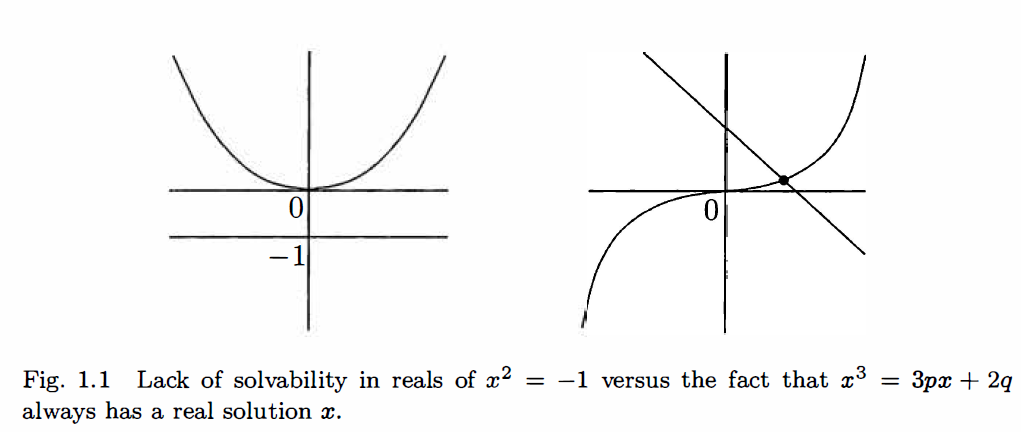
\includegraphics[width=0.6\textwidth]{./SaltChapter/fig-1-1}
\end{center}
\caption{실근이 존재하지 않는 방정식 $x^2=-1$과 항상 실근을 갖는 $x^3=3px+2q$}
\label{fig-1-1}
\end{figure}

Cardano (1501-1576)는 3차방정식 $x^3=3px+2q$의 실근을 구하는 다음 공식을 만들었다.
$$
x = \sqrt[3]{q+ \sqrt{q^2-p^3}} + \sqrt[3]{q- \sqrt{q^2-p^3}}
$$
예를 들어, $p=2$, $q=3$일 때 방정식 $x^3=6x+6$은 $x=\sqrt[3]{4}+\sqrt[3]{2}$를 해로 가진다.
한편, 중간값 정리에 의해 3차함수 $y=x^3$은  항상 $y=3px+2q$와 만난다.
그림 \ref{fig-1-1}의 오른쪽 그래프를 참고하라.
하지만 $p=5$, $q=2$로 방정식 $x^3=15 x+4$을 만들면 $q^2-p^3= -121<0$이 되어
실수만으로는 Cardano의 공식을 적용하지 못한다.
그럼에도 불구하고 우리는 $x=4$가 실근이 됨을 확인할 수 있다.
$$
4^3 = 64 = 60 + 4 = 15\cdot 4 + 4.
$$
Cardano 공식이 나온지 30년 후, Bombelli가 복소수 연산을 도입하면
Cardano 공식으로 원하는 실근을 도출할 수 있음을 제안하였다.
다음 등식이 성립할 수 있을까?
$$
x = \sqrt[3]{2+11i} + \sqrt[3]{2-11i} \stackrel{?}{=} 4.
$$
$(2+i)^3 = 2+11i$이고 $(2-i)^3 = 1-11i$임을 이용하면
세제곱근 값으로부터 위 등식이 성립함을 알 수 있다.
따라서 Bombelli의 결과로부터 실수 문제에도 복소수 연산이 연결될 수 있음이 입증되었다.
그때부터 복소수가 수학의 주류에 들어가게 되었다.

\begin{salt_exercise} \label{ex-1-3}
양의 부분집합 $P\subset \mathbb F$가 있어 다음을 만족하면
체 $\mathbb F$는 순서(ordered)를 갖는다고 한다.
\begin{itemize}
\item[(P1)] 모든 $x,y\in P$에 대하여, $x+y\in P$.
\item[(P2)] 모든 $x,y\in P$에 대하여, $x\cdot y \in P$
\item[(P3)] 모든 $x\in P$에 대하여, 다음 3가지 중  정확히 한가지만 참이다.
$$
1^{\circ} \ x=0. \quad 2^{\circ} \ x\in P. \quad 3^{\circ} \ -x\in P.
$$
\end{itemize}
예를 들면, $P:=(0,\infty)$를 양의 부분집합이라 하면
실수체 $\mathbb R$은 순서를 갖는다.
( 순서를 갖는 체 $\mathbb F$에서 두 원소 $x,y\in \mathbb F$의 관계 $>_P$를
$y>_P x$는 $y-x \in P$로 정의하여 대소관계를 정할 수 있다.)
복소수 $\mathbb C$는 순서를 가질 수 없음을 보여라. \\[1ex]
힌트: $x:=i$에 대하여 $x\cdot x$를 살펴보라.
\end{salt_exercise}

\section{복소수의 기하학적 표현}

$\mathbb C = \mathbb R^2$이므로, 
그림 \ref{fig-1-2}와 같이 복소수를 평면위의 점에 대응시킬 수 있다.

\begin{figure}[!h]
\begin{center}
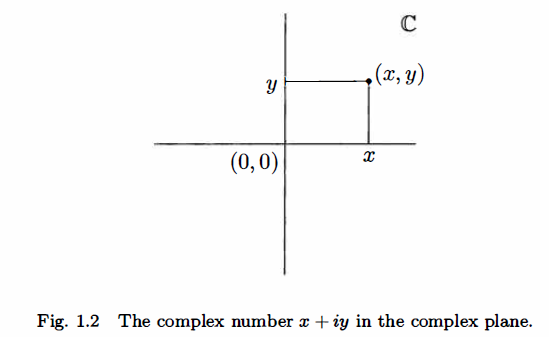
\includegraphics[width=0.5\textwidth]{./SaltChapter/fig-1-2}
\end{center}
\caption{복소평면에 표시한 복소수 $x+iy$}
\label{fig-1-2}
\end{figure}

복소평면은 Argrand\footnote{ 
Jean-Robert Argand (1768-1822)의 이름에서 따온 것이다.
Caspar Wessel (1745-1818)이 더 먼저 사용하긴 했으나.}
평면이라고도 불린다.

\begin{salt_exercise} \label{ex-1-4}
다음 복소수를 복소평면 위의 점으로 표시하라.
$$
0, \quad 1 , \quad -\frac32, \quad i, \quad -\sqrt{2}i,
\quad \cos \frac\pi3 + i\sin\frac\pi3.
$$
\end{salt_exercise}

따라서 복소수 $\mathbb C$는 {\bf 집합}으로서 평면 $\mathbb R^2$로 간주할 수 있다.
$\mathbb C$에 정의된 체의 연산이 평면에서 기하학적 의미를 가질까?
우리는 앞으로 실제로 의미가 있음을 살펴볼 것이다.
$\mathbb C$의 덧셈은 평면벡터의 덧셈이고
곱셈은 조금 더 특별한 의미를 갖는다.

{\bf 복소수 덧셈의 기하학적 의미: }
복소수를 평면 위의 점으로 간주하고 복소수의 덧셈을 $\mathbb R^2$의 벡터 합으로 
정의하는 것이 자연스럽다. 
벡터 합은 두 벡터를 결합하는 일반적인 방식으로 정의한다.
즉, $(0,0)$과 두 복소수를 잇는 선분으로 이루어진 평생사변형을 완성시킬 때
$(0,0)$과 대각선의 반대에 있는 점을 두 복소수의 합이 된다.
그림 \ref{fig-1-3}\을 참고하라.

\begin{figure}[!h]
\begin{center}
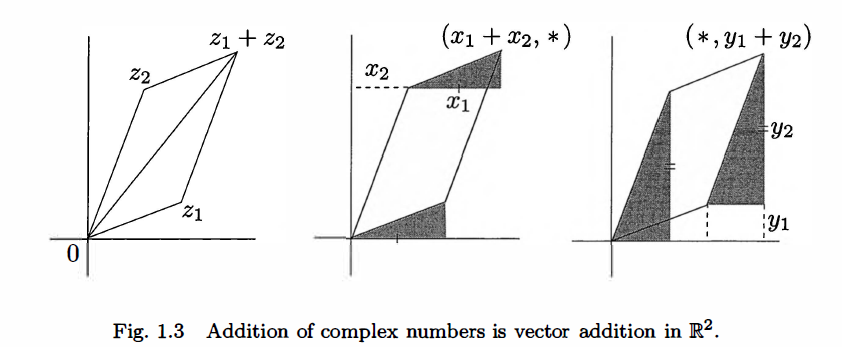
\includegraphics[width=0.8\textwidth]{./SaltChapter/fig-1-3}
\end{center}
\caption{복소수 덧셈은 $\mathbb R^2$의 벡터 합이다.}
\label{fig-1-3}
\end{figure}

{\bf  복소수 곱셈의 기하학적 의미: }
이제 복소수 곱셈이 가진 특별한 기하학적 의미를 살펴보자.
이를 위해 편의상 극좌표를 사용한다.
$(x,y)\in\mathbb R^2$이 극좌표 $r\ge 0$와 $\theta\in(-\pi,\pi]$로 표현된다고 하자.
이는 원점에서 $(x,y)$까지의 거리를 $r(\ge0)$이고,
$(0,0)$에서 $(x,y)$를 잇는 반직선이 $x$-축의 양의 방향과 이루는 각이 $\theta$가 된다는 뜻이다.
($(x,y)$가 원점 $(0,0)$인 경우, $\theta=0$으로 정한다.)

\begin{figure}[!h]
\begin{center}
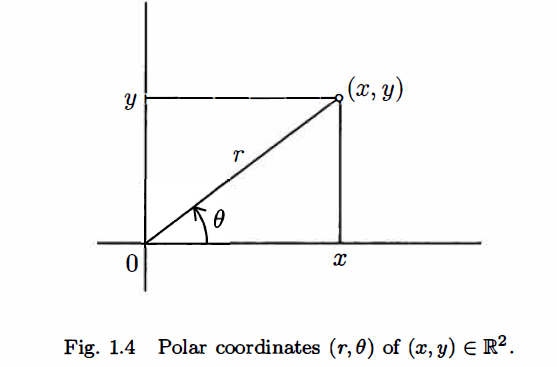
\includegraphics[width=0.5\textwidth]{./SaltChapter/fig-1-4}
\end{center}
\caption{복소수 $(x,y)\in\mathbb R^2$의 극좌표 표현 $(r, \theta)$}
\label{fig-1-4}
\end{figure}

그림 \ref{fig-1-4}의 직각삼각형으로부터 다음 관계를 얻는다.
\begin{gather*}
x = r \cos\theta, \\
y = r \sin \theta.
\end{gather*}
이로부터 복소수를 극좌표 $(r,\theta)$로 표현할 수 있다.
$$
x + yi = r\cos\theta +(r\sin \theta)i
= r(\cos\theta + i\sin \theta).
$$
이제 복소수 곱셈의 기하학적으로 해석하자.
두 복소수를 모두 극좌표로 쓰면
\begin{gather*}
z_1 = r_1 (\cos\theta_1 + i\sin\theta_1), \\
z_2 = r_2 (\cos\theta_2 + i\sin\theta_2),
\end{gather*}
삼각함수의 덧셈정리로부터 다음을 얻는다.
\begin{align*}
z_1\cdot z_2 &= r_1(\cos\theta_1+i\sin\theta_1) \cdot r_2(\cos\theta_2+i\sin\theta_2) \\
&= r_1r_2 (\cos\theta_1\cos\theta_2 - \sin\theta_1\sin\theta_2 +
i(\cos\theta_1\sin\theta_2 + \cos\theta_2\sin\theta_1)) \\
&= r_1r_2(\cos(\theta_1 +\theta_2) + i \sin(\theta_1 +\theta_2)).
\end{align*}
따라서 $z_1\cdot z_2$는 극좌표로 $(r_1r_2, \theta_1+\theta_2)$이다.
다시 말하면, 
$z_1\cdot z_2$의 편각은
$z_1$과 $z_2$가 각각 실수축의 양의 방향과 이루는 각을 더하여 얻을 수 있고,
원점에서의 거리는 각각의 거리를 곱하여 얻는다.
그림 \ref{fig-1-5}\를 참고하라.

\begin{figure}[!h]
\begin{center}
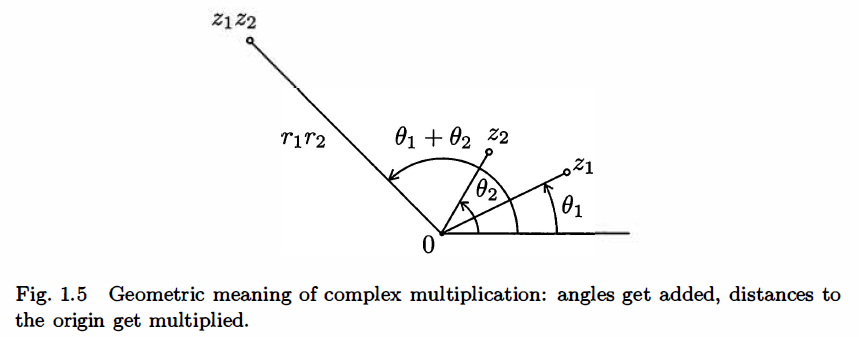
\includegraphics[width=0.5\textwidth]{./SaltChapter/fig-1-5}
\end{center}
\caption{복소수 곱셈의 기하학적 의미: 각은 더하고, 원점에서의 거리는 곱한다.}
\label{fig-1-5}
\end{figure}

특별한 경우로 원점에서의 거리가 $1$인 복소수
$\cos\alpha + i \sin\alpha$를 곱하는 경우를 생각해보자.
그러면 위의 식으로부터 $z\in\mathbb C$와의 곱
$z\cdot(\cos\alpha + i\sin\alpha)$는 
원점과 $z$를 연결하는 직선을 반시계방향으로 $\alpha$만큼 회전시켜 얻을 수 있다.
특히, $z$에 
$$
i = 0 + i\cdot 1 = \cos\frac\pi2 + i \sin\frac\pi2
$$
를 곱하면 반시계방향으로 $90^{\circ}$ 회전한 결과를 얻는다.

\begin{figure}[!h]
\begin{center}
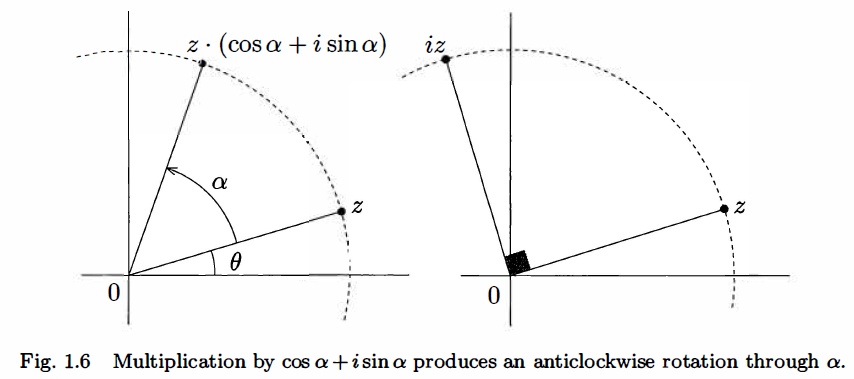
\includegraphics[width=0.8\textwidth]{./SaltChapter/fig-1-6}
\end{center}
\caption{$\cos\alpha + i \sin\alpha$를 곱하면 반시계방향으로 $\alpha$만큼 회전한 결과를 얻는다.}
\label{fig-1-6}
\end{figure}

{\bf 드 므와브르(De Moivre) 정리와 $n$차 제곱근 :}
모든 자연수 $n\in\mathbb N$에 대하여
$$
(\cos\theta + i\sin\theta)^n = \cos(n\theta) + i\sin(n\theta)
$$
가 성립하며 이를 드 므와브르 정리라 한다.

\begin{salt_exercise} \label{ex-1-5}
드 므와브르의 정리를 이용하여
삼각함수의 3배각 공식 $\cos (3\theta) = 4(\cos\theta)^3 - 3\cos\theta$을 증명하라.
\end{salt_exercise}

\begin{salt_exercise} \label{ex-1-6}
$(1+i)^{10}$을 직접 전개하지 않고 $x+iy$ ($x,y$는 실수)의 꼴로 써라?
\end{salt_exercise}

\begin{salt_exercise} \label{ex-1-7}
$(2+i)(3+i)$를 이용하여
$\dfrac\pi4 = \tan^{-1}\dfrac12 + \tan^{-1}\dfrac13$을 증명하다.
\end{salt_exercise}

\begin{salt_exercise} \label{ex-1-8}
가우스 정수(Gaussian integer)는 
$m, n$이 정수일 때, $m+in$꼴의 복소수로
복소평면 위의 정수 격자점을 이룬다.
모든 꼭지점이 가우스 정수가 되도록 정삼각형을 그리는 것을 불가능함을 증명하라. \\[1ex]
힌트: 한변의 회전으로 다른 변을 만들 수 있고, $\sqrt{3}\not\in \mathbb Q$임을 이용하라.
\end{salt_exercise}

드 므와브르 공식을 이용하면
복소수  $z$의 $n$ 제곱근
즉, $w^n=z$를 만족하는 복소수 $w$를 쉽게 구할 수 있다.
우선 적당한 $r\ge0$과 $\theta\in[0,2\pi)$에 대하여 $z=r(\cos\theta + i \sin\theta)$로 쓰자.
$w= \rho(\cos\alpha + i\sin\alpha)$가 $w^n=z$를 만족한다면,
$$
w^n = \rho^n\left( \cos(n\alpha) + i\sin(n\alpha)\right) = r(\cos\theta + i\sin\theta)= z.
$$
양변은 원점에서의 거리가 같으므로 $\rho^n=r$을 얻는다.
$\rho$와 $r$이 음수가 아니므로 $\rho = \sqrt[n]{r}$이다.
한편 $w^n$이 실수축의 양의 방향과 이루는 각 $n\alpha$는 
집합 $ \{ \ldots, \theta - 4\pi, \theta - 2\pi, \theta, \theta+2\pi, \theta+4\pi, \ldots\} $에 속한다.
$0$이 아닌 $z$가 실수축의 양의 방향과 이루는 각은 $2\pi$의 정수배 차이를 무시하면 유일하게 결정되므로
$\theta$ 대신 $\theta + 2\pi k$ ($k$는 정수)로도 쓴다. 그림 \ref{fig-1-7}\을 참고하라.

\begin{figure}[!h]
\begin{center}
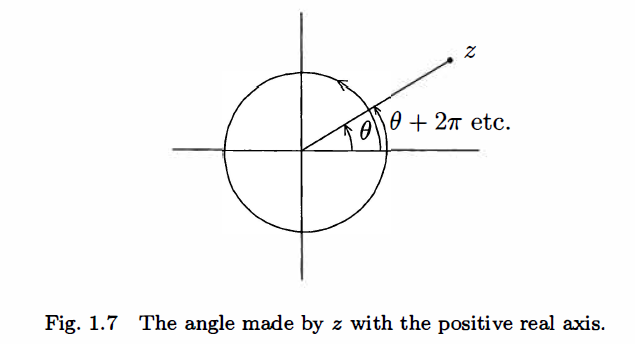
\includegraphics[width=0.7\textwidth]{./SaltChapter/fig-1-7}
\end{center}
\caption{복소수 $z$가 실수축의 양의 방향과 이루는 각}
\label{fig-1-7}
\end{figure}

이제 $\alpha \in \left\{ \dfrac{\theta}{n}+ \dfrac{2\pi}{n}k \,:\, k\in\mathbb Z \right\}$로부터
서로 다른 $w$가 되는 $\alpha$만 쓰면 다음과 같다.
$$
\alpha \in \left\{
\dfrac\theta n,  \dfrac\theta n+ \dfrac{2\pi}n, \dfrac\theta n + 2\cdot \dfrac{2\pi}n, \ldots,
\dfrac\theta n+ (n-1)\cdot \dfrac{2\pi}n
\right\}.
$$
특히, $z=1$일 때, $1$의 $n$제곱근은 원에 내접하는 정$n$각형의 꼭지점이다.
그림 \ref{fig-1-8}을 보라.
\begin{figure}[!h]
\begin{center}
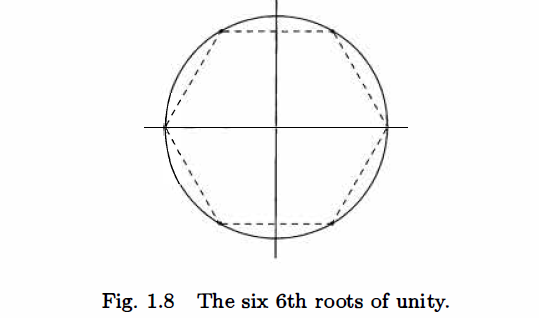
\includegraphics[width=0.7\textwidth]{./SaltChapter/fig-1-8}
\end{center}
\caption{$1$의 $6$ 제곱근 $6$개}
\label{fig-1-8}
\end{figure}

\begin{salt_exercise} \label{ex-1-9}
$w^4=-1$을 만족하는 모든 복소수 $w$를 찾아
복소평면에 표시하라.
\end{salt_exercise}

\begin{salt_exercise} \label{ex-1-10}
$z^6-z^3-2=0$을 만족하는 모든 복소수 $z$를 구하라.
\end{salt_exercise}

\begin{salt_exercise} \label{ex-1-11}
$a^2+b^2+c^2= ab+bc+ca$를 만족하는 실수 $a,b,c$는 모두 같다.
실제로 양변에 $2$를 곱하고 정리하면
$(a-b)^2+(b-c)^2+(c-a)^2=0$을 얻고, 
각 항은 음수가 아니므로 모두 $0$이 될 수밖에 없다.
한편, $a^2+b^2+c^2= ab+bc+ca$를 만족하는 복소수 $a,b,c$는
복소평면위의 정삼각형의 꼭지점이 됨을 보여라.
실수의 경우와 결과를 비교하라. \\[1ex]
힌트: 실수가 아닌 $1$의 세제곱근 $\omega$에 대하여
$((b-a)\omega + (b-c))\cdot((b-a)\omega^2 + (b-c))$를 계산하라.
\end{salt_exercise}

\begin{salt_exercise} \label{ex-1-12}
이항정리에서
$a,b$가 실수이고, $n\in\mathbb N$이면,
$$
(a+b)^n = \sum_{k=0}^n {n \choose k}a^kb^{n-k},
\quad
\text{여기서 }
{n \choose k} := \frac{n!}{k!(n-k)!}, \
k=0,1,2,\ldots, n,
$$
는 이항계수라 한다.
대수적 연산을 생각하면 이 등식은 $a,b$가 복소수인 경우에도 성립한다.
$$
{3n \choose 0} + {3n \choose 3} + {3n \choose 6} + \cdots
+ {3n \choose 3n} = \dfrac{2^{3n} + 2\cdot(-1)^n}3
$$
이 성립함을 보여라. \\[1ex]
힌트: $\omega$가 실수가 아닌 $1$의 세제곱근일 때
$(1+1)^{3n} + (1+\omega)^{3n} + (1+\omega^2)^{3n}$을 계산하라.
\end{salt_exercise}

\begin{salt_exercise} \label{ex-1-13}
복소수의 기하학적 성질을 이용하여 
사각형의 대변에 외접하는 정사각형 중심을 잇는 두 선분은
길이가 같고, 수직으로 만남을 증명하라.
\end{salt_exercise}

{\bf 절대값과 켤레복소수: }
복소수 $z=x+iy$ ($x,y\in\mathbb R$)의 절대값 $|z|$는
$$
|z| = \sqrt{x^2+y^2}
$$
로 정의한다.
피타고라스 정리에 따라 이는 $z$와 원점 사이의 거리를 나타낸다.
그림 \ref{fig-1-9}의 왼쪽을 참고하라.
$z_1, z_2\in \mathbb C$를 극좌표로 쓰거나, 직접 계산하여 확인하면
$|z_1z_2| = |z_1|\cdot |z_2|$임을 쉽게 확인할 수 있다.

\begin{figure}[!h]
\begin{center}
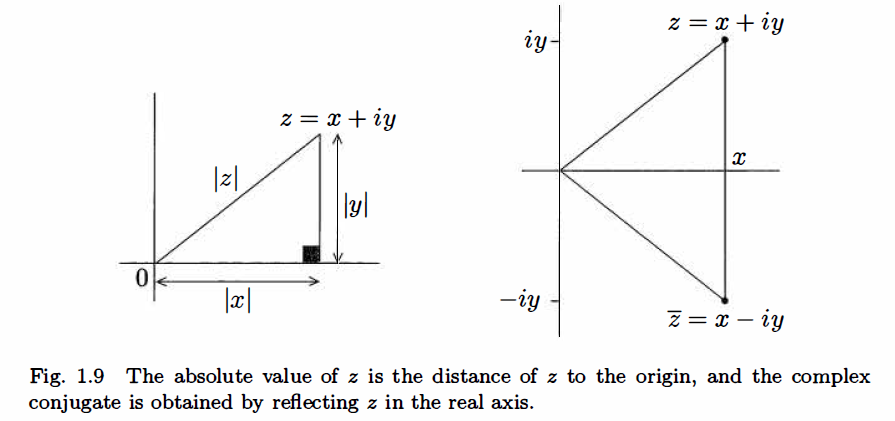
\includegraphics[width=0.7\textwidth]{./SaltChapter/fig-1-9}
\end{center}
\caption{복소수의 절대값은 원점에서의 거리이고, 켤레복소수는 실수축에 대칭인 복소수이다.}
\label{fig-1-9}
\end{figure}

\begin{salt_exercise} \label{ex-1-14}
직표좌표로 $z_1, z_2$를 써서 $|z_1z_2| = |z_1|\cdot |z_2|$임을 확인하라.
\end{salt_exercise}

복소수 $z=x+iy$ ($x,y\in\mathbb R$)의 켤레복소수 $\bar z$는
$$
\bar z = x - iy
$$
로 정의한다.
복소평면에서 $\bar z$는 $z$를 실수축으로 대칭시켜 얻는다.
그림 \ref{fig-1-9}의 오른쪽을 참고하라.
기하학적 표현으로부터 복소수 $z_1, z_2\in\mathbb C$에 대하여
다음이 성립함을 확인할 수 있다.
$$
\overline{z_1+z_2} = \overline{z_1} + \overline{z_2},
\quad
\overline{z_1\cdot z_2} = \overline{z_1} \cdot \overline{z_2}.
$$

다음 성질도 쉽게 얻을 수 있다.
$$
\bar{\bar z} = z, \quad z\bar z  = |z|^2 \quad
\Re(z) = \frac{z+\bar z}2, \quad \Im(z) = \frac{z-\bar z}{2i}.
$$

\begin{salt_exercise} \label{ex-1-15}
위의 등식 4개를 증명하라.
\end{salt_exercise}

\begin{salt_exercise} \label{ex-1-16}
모든 복소수 $z\in\mathbb C$에 대하여
$|z|=|\bar z|$, $|\Re(z)|\le |z|$, $|\Im(z)| \le |z|$임을 증명하고
각각에 대하여 기하학적으로 설명하라.
\end{salt_exercise}

\begin{salt_exercise} \label{ex-1-17}
$|a|<1$과 $|z|\le 1$을 만족하는 $a,z\in\mathbb C$에 대하여
$\left| \dfrac{z-a}{1-\bar a z}\right| \le 1$을 보여라.
\end{salt_exercise}

\begin{salt_exercise} \label{ex-1-18}
계수가 $c_0, c_1, \ldots, c_d\in\mathbb R$이고 $c_d\ne0$인 다항식
$p(z) = c_0+c_1z+\cdots + c_dz^d$을 생각하자.
$w\in\mathbb C$가 $p(w)=0$을 만족하면 $p(\bar w)=0$도 성립함을 보여라.
\end{salt_exercise}

\begin{salt_exercise} \label{ex-1-19}
복소수 $0, a, b \in\mathbb C$가 만드는 삼각형의 면적은
$\left| \dfrac{\Im(a\bar b)}2\right|$임을 보여라.
\end{salt_exercise}

\begin{salt_exercise} \label{ex-1-20}
임의의 복소수 $z_1,z_2, z_3$에 대하여
$i\det \begin{pmatrix}
1 & z_1 & \overline{z_1} \\
1 & z_2 & \overline{z_2} \\
1 & z_3 & \overline{z_3} 
\end{pmatrix}$는 실수임을 증명하라.
\end{salt_exercise}

\begin{salt_exercise} \label{ex-1-21}
임의의 두 복소수 $z_1, z_2$가
$|z_1+z_2|^2 + |z_1-z_2|^2 =2(|z_1|^2+|z_2|^2)$을 만족함을 보여라.
이 등식의 기하학적 의미는 무엇인가?
\end{salt_exercise}

\section{$\mathbb C$의 위상}

실수 $\mathbb R$에서 수열의 수렴성, 함수의 연속성과 미분가능성과 같은
일반적인 미적분 개념들은 모두 실수에서 점의 가까움에 대한 개념에 의존한다.
예를 들면, 실수열 $(a_n)_{n\in\mathbb N}$의 극한이 $L\in\mathbb R$이라는 것은,
주어진 양수 $\epsilon$에 대하여 충분히 큰 인덱스 $N$이 있어 이를 넘는 인덱스를 갖는
 $a_n$은 모두 $L$과의 {\bf 거리}가 기껏해야 $\epsilon$이하임을 의미한다.
``$a_n$과  $L$의 거리''는 $|a_n-L|$로 정의하며
실수 라인에서 $a_n$과 $L$을 잇는 선분의 길이를 뜻한다.

이제 {\bf 복소수}에서 미적분을 만들어 보려면
복소수 쌍 $(z_1, z_2)$에 대한 거리 $d(z_1, z_2)$의 개념이 필요하다.
첫 단계로 거리의 개념이 무엇인지 살펴보자.

\subsection{$\mathbb C$에서의 거리 개념}

복소수 $\mathbb C$를 $\mathbb R^2$으로 보면 $\mathbb R^2$의 유클리드 거리로
$\mathbb C$의 거리를 정의할 수 있다.
따라서, 복소수 $z_1=x_1+iy_1$과 $z_2=x_2+iy_2$에 대하여 
다음 식으로 거리를 정의한다.
$$
d(z_1,z_2) = \sqrt{(x_1-x_2)^2 + (y_1+y_2)^2} = |z_1-z_2|.
$$
피타고라스 정리에 의하여 이 값은 $\mathbb R^2$ 평면의 두 점 $(x_1, y_1)$과 $(x_2, y_2)$의 거리와 같다.
그림 \ref{fig-1-10}을 참고하라.

\begin{figure}[!h]
\begin{center}
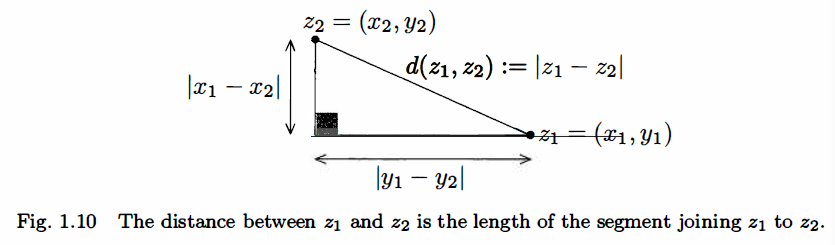
\includegraphics[width=0.9\textwidth]{./SaltChapter/fig-1-10}
\end{center}
\caption{복소수 $z_1$과 $z_2$사이의 거리는 $z_1$과 $z_2$를 잇는 선분의 길이다.}
\label{fig-1-10}
\end{figure}

복소수 덧셈의 기하학적 의미와 
삼각형의 두변의 길이의 합은 가장 큰 변의 길이보다 크다는 
유클리드 기하학의 유명한 결과를 이용하면
다음과 같이 복소수 절대값의 삼각 부등식을 얻는다.
$$
|z_1+z_2| \le |z_1|  + |z_2|, \quad z_1, z_2\in\mathbb C.
$$

그림 \ref{fig-1-11}을 보자.
이 삼각 부등식은 실수 $x_1, x_2, y_1, y_2$에 대한 코시-슈바르츠 부등식
$(x_1^2+y_1^2) (x_2^2+y_2^2) \ge (x_1x_2 + y_1y_2)^2$을 사용하여
확인할 수도 있다.


\begin{figure}[!h]
\begin{center}
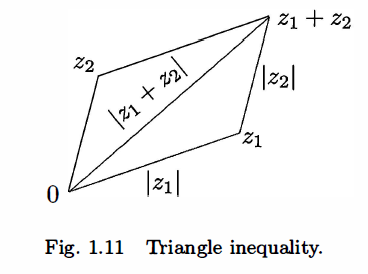
\includegraphics[width=0.5\textwidth]{./SaltChapter/fig-1-11}
\end{center}
\caption{삼각 부등식}
\label{fig-1-11}
\end{figure}

\begin{salt_exercise} \label{ex-1-22}
모든 복소수 $z_1, z_2\in \mathbb C$에 대하여
$|z_1-z_2| \ge \left| |z_1| - |z_2| \right|$을 증명하라.
\end{salt_exercise}

\begin{salt_exercise} \label{ex-1-23}
다음 집합을 복소평면에 나타내라.
\begin{itemize}
\item[(1)] $\left\{z\in\mathbb C\,:\, |z-(1-i)| = 2 \right\}$.
\item[(2)] $\left\{z\in\mathbb C\,:\, |z-(1-i)| < 2 \right\}$.
\item[(3)] $\left\{z\in\mathbb C\,:\, 1< |z-(1-i)| < 2 \right\}$.
\item[(4)] $\left\{z\in\mathbb C\,:\, \Re(z-(1-i)) = 3 \right\}$.
\item[(5)] $\left\{z\in\mathbb C\,:\, |\Im(z-(1-i))| < 2 \right\}$.
\item[(6)] $\left\{z\in\mathbb C\,:\, |z-(1-i)| = |z-(1+i)| \right\}$.
\item[(7)] $\left\{z\in\mathbb C\,:\, |z-(1-i)| + |z-(1+i)| = 2 \right\}$.
\item[(8)] $\left\{z\in\mathbb C\,:\, |z-(1-i)| + |z-(1+i)| < 3 \right\}$.
\end{itemize}
\end{salt_exercise}

\subsection{열린 원판, 열린 집합, 닫힌 집합, 콤팩트 집합}

주어진 점의 근방에 대한 집합을 다루기 위해 다음 정의들을 도입하는 것이 편리하다.
중심이 $z_0$이고 반지름이 $r>0$인 {\bf 열린 공/원판} $D(z_0,r)$은 
$D(z_0,r) :=\{ z\in\mathbb C \,:\, |z-z_0| <r \}$로 정의한다.

\begin{figure*}[!h]
\begin{center}
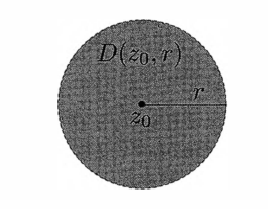
\includegraphics[width=0.3\textwidth]{./SaltChapter/fig-1-0-1}
\end{center}
\end{figure*}

$\mathbb C$의 부분집합 $U$에 속하는
모든 $z$에 대하여 $r_z>0$가 존재하여 $D(z,r_z)\subset U$를 만족하면
$U$를 {\bf 열린 집합}이라 한다.
다시 말하면, $U$의 어떤 점을 잡더라도 
주변의 모든 점이 $U$에 속할 수 있는 ``공간''이 존재한다.
예를 들면, 열린 원판 $D(z_0,r)$은 열린 집합이다.
따라서  $D(z_0,r)$를 열린 원판이라 부를 때 사용한 형용사 ``열린''은 적절해 보인다.
열린 집합의 예를 조금 더 만들어보자.
원환(annulus) $\mathbb A_r := \{ z\in\mathbb C\,:\, r<|z|<1\}$,
우측 반평면 $\mathbb H:= \{z\in\mathbb C\,:\, \Re(z)>0\}$는 모두 열린 집합이다.

열린 집합의 여집합에 특별한 이름을 붙여 ``닫힌 집합''이라 부르면 편리하다.
닫힌 집합은 수열의 수렴성의 관점에서 규정할 수도 있다.
집합 $F\subset \mathbb C$가 닫힌 집합이라는 것은
$F$에 속하는 복소수열 $(z_n)_{n\in\mathbb N}$이  $\mathbb C$에서 $L$로 수렴한다면
극한 $L$이 $F$에 속한다는 것과 동치이다.

$\mathbb C$의 부분집합 $S$의 모든 원소 $z$에 대하여
$|z|\le M$을 만족하는 $M>0$이 존재하면 $S$를 {\bf 유계}(bounded)라 한다.
그러면 $S$는 복소평면에서 충분히 큰 원판 내부에 속한다.

$\mathbb C$의 부분집합 $K$가 유계인 닫힌 집합이면 {\bf 콤팩트 집합}이라 한다.
콤팩트 집합에서 정의된 실변수 연속함수는 최대값과 최소값을 갖는다는
실해석학의 잘 알려진 결과를
앞으로 종종 사용할 것이다.

\subsection{수렴성과 연속성}

$\mathbb C$에서 수열의 수렴성에 대하여 알아보자.
 
복소수열 $(z_n)_{n\in\mathbb N}$이 수렴하고 극한이 $L$이라는 것은
임의의 $\epsilon>0$에 대하여 인덱스 $N\in\mathbb N$이 존재하여
모든 $n>N$에 대하여 $|z_n -L| < \epsilon$이 성립함을 의미한다.
삼각 부등식에 의하여 수렴하는 수열의 극한은 유일하게 결정되며
다음과 같이 쓴다.
$$
\lim_{n\to\infty} z_n = L.
$$

\begin{saltexample}{}{} \label{example-1-1}
복소수 $z$가 $|z|<1$를 만족한다고 하자.
그러면 수열 $(z_n)_{n\in\mathbb N}$은 $0$으로 수렴한다.
왜냐하면, $|z^n-0| = |z^n| = |z|^n = ||z|^n-0|$인데
$|z|<1$이므로, $n\to\infty$일 때 $|z|^n\to0$이기 때문이다.
\end{saltexample}

\begin{salt_exercise} \label{ex-1-24}
복소수 계수 $c_0, c_1, \ldots, c_d\in \mathbb C$의
다항식 $p(z)=c_0 + c_1z + \cdots + c_dz^d$ ($c_d\ne0$)를 생각하자.
$|z|>R$인 모든 $z$에 대하여 $|p(z)| \ge M|z|^d$을 만족하는
$M, R>0$이 존재함을 증명하라.
\end{salt_exercise}

\begin{salt_exercise} \label{ex-1-25}
복소수열 $(z_n)_{n\in\mathbb N}$이 $L$로 수렴함과
실수열 $(\Re(z_n))_{n\in\mathbb N}$과  $(\Im(z_n))_{n\in\mathbb N}$이
각각 $\Re(L)$과 $\Im(L)$로 수렴함이 동치임을 보여라.
\end{salt_exercise}

\begin{salt_exercise} \label{ex-1-26}
복소수열 $(z_n)_{n\in\mathbb N}$이 $L$로 수렴함과
$(\overline{z_n})_{n\in\mathbb N}$이 $\bar L$로 수렴함은 동치임을 보여라.
\end{salt_exercise}

\begin{salt_exercise} \label{ex-1-27}
$\mathbb C$가 완비성(completeness)을 가짐을 증명하라.
즉, $\mathbb C$의 모든 코시 수열이 $\mathbb C$의 원소로 수렴한다.
(임의의 $\epsilon>0$에 대하여 인덱스 $N\in\mathbb N$이 존재하여
$m,n>N$ 이면, $|z_n - z_m| < \epsilon$을 만족할 때
수열 $(z_n)_{n\in\mathbb N}$을 {\bf 코시 수열}이라 한다.
)
\end{salt_exercise}

$S$가 $\mathbb C$의 부분집합, $z_0\in S$,  $f:S\to \mathbb C$라 하자.
임의의 $\epsilon>0$에 대하여 $\delta>0$가 존재하여
$z\in S$가 $|z-z_0|<\delta$를 만족하면 $|f(z)-f(z_0)|<\epsilon$일 때
$f$는 $z_0$에서 {\bf 연속}이라고 한다.

수열의 극한으로도 연속성을 규정할 수 있다.
$f:S\to\mathbb C$가 $z_0$에서 연속임은
$z_0$로 수렴하는 $S$의 모든 복수열 $(z_n)_{n\in\mathbb N}$에 대하여
$(f(z_n))_{n\in\mathbb N}$이 $f(z_0)$로 수렴함과 동치이다.

\begin{saltexample}{}{} \label{example-1-2}
켤레복소수를 만드는 것은 연속함수이다.
즉, $z\to\bar z: \mathbb C \to \mathbb C$는 연속이다.
모든 $z, z_0 \in \mathbb C$에 대하여
$|\bar z - \overline{z_0}| = |\overline{z-z_0}| = |z-z_0|$이다.
이로부터 모든 $z_0\in\mathbb C$에 대하여 켤레복소수를 대응시키는 함수는
연속이다. 기하학적으로 보면 자명하다. 왜냐 하면, 켤레복소수는 단지 실수축에 대하여 
대칭시키는 것이므로 가까운 두 점은 함수값도 가까이 머물기 때문이다!

모든 $z\in\mathbb C$에 대하여 $\overline{(\bar z)} = z$ 켤레복소수의
역함수는 자기자신이다. 따라서 켤레복소수는 가역이며 역함수도 연속이다.
따라서 켤레복소수 함수는 $\mathbb C$에서 $\mathbb C$로의 
위상동형사상(homeomorphism)이다 (연속인 전단사함수이며 역함수도 연속이다).
\end{saltexample}

\begin{salt_exercise} \label{ex-1-28}
함수 $z\mapsto \Re(z): \mathbb C \to \mathbb R$은 연속함수임을 증명하라. 
\end{salt_exercise}

\subsection{영역}

이후에는  경로연결된 열린 집합의 개념이 중요한 역할을 한다.
우리 학습의 주요 대상, 즉, 집합 $D(\subset \mathbb C)$의 모든 점에서
복소미분 가능함수 $f:D\to\mathbb C$에 대한 결과를 증명할 때 사용된다.
많은 정리들이 유효하게 성립하려면 $D$가 $\mathbb C$의 ``좋은'' 부분집합이 되어야 하며
단순히 $\mathbb C$의 부분집합이라는 조건만으로는 부족함을 보게 될 것이다.
``좋음''이라는 가정을 만족하는 집합을 영역이라 부르며 정확히는 다음과 같이 규정된다.

우리는 $\mathbb C$의 경로연결된 열린 부분집합을 영역(domain)이라 부른다.
``열린''의 의미는 이미 알고 있으니 ``경로연결된''이 어떤 의미인지 설명해보자.

\begin{saltdefinition}{}{} \label{def-1-1}

\begin{itemize}
\item[(1)] 연속함수 $\gamma:[a,b] \to \mathbb C$를 $\mathbb C$의 경로(또는 곡선)이라 한다.
%\begin{figure*}[!h]
\begin{center}
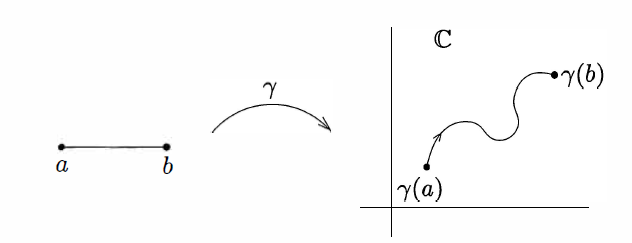
\includegraphics[width=0.5\textwidth]{./SaltChapter/fig-1-0-2}
\end{center}
%\end{figure*}
\item[(2)] 경로 $\gamma:[a,b] \to \mathbb C$가 다음 조건을 만족하면 계단식 경로(stepwise path)라 한다.
점 $t_0 = a < t_1 < \cdots < t_n < t_{n+1} = b$가 존재하여
부분경로 $\gamma: [t_k, t_{k+1}] \to \mathbb C$ ($k=0,1,\ldots, n$)가
실수부가 상수 또는 허수부가 상수인 경로가 된다.
%\begin{figure*}[!h]
\begin{center}
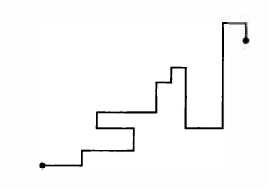
\includegraphics[width=0.3\textwidth]{./SaltChapter/fig-1-0-3}
\end{center}
%\end{figure*}
\item[(3)] $U$가 열린 집합일 때,  모든 $z_1, z_2\in U$에 대하여
$\gamma(a)=z_1$, $\gamma(b)=z_2$이고 모든 $t\in[a,b]$에서 $\gamma(t)\in U$인
계단식 경로 $\gamma: [a,b] \to \mathbb C$가 존재하면
$U$를 경로연결된 열린 집합이라 한다.
\end{itemize}
\end{saltdefinition}

실제로 위에서 경로연결된 열린 집합을 정의할 때 경로를 {\bf 계단식} 경로에 한정한 것을 
완화할 수 있다. 즉, 열린 집합에 포함된 임의의 두 점이 집합내의 경로로 연결되기만 하면
경로연결된 것으로 정의해도
우리가 정의한 경로연결된 집합과 일치한다.
하지만 우리에게는 불필요한 일반화이며, 앞에서 정의한 것으로 충분하다.

\begin{saltexample}{}{} \label{example-1-3}
\
\begin{itemize}
\item[(1)] 열린 단위원판 $\mathbb D := \{ z\in\mathbb C\,:\, |z|<1 \}$은 영역이다.
\item[(2)] $r\in (0,1)$에 대하여 원환 $\mathbb A_r := \{ z\in\mathbb C\,:\, r<|z|<1\}$은 영역이다.
\item[(3)] 우측 반평면 $\mathbb H := \{ z\in \mathbb C \,:\, \Re(z)>0\}$은 영역이다.
\end{itemize}

%\begin{figure}[!h]
\begin{center}
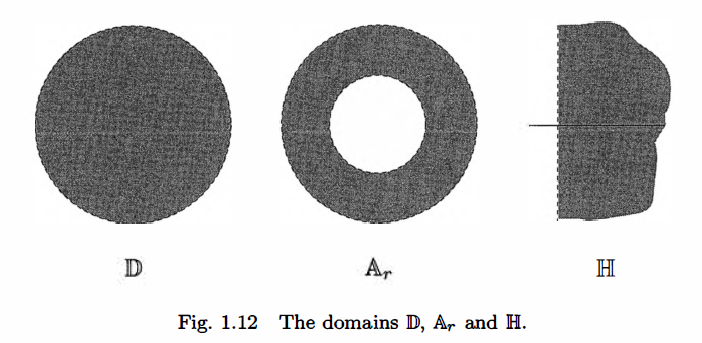
\includegraphics[width=0.7\textwidth]{./SaltChapter/fig-1-12}
\end{center}
\captionof{figure}{영역 $\mathbb D$, $\mathbb A_r$, $\mathbb H$}
\label{fig-1-12}
%\end{figure}
\end{saltexample}

한편, 집합 $S:=\{z\in\mathbb C \,:\, |z|\ne 1\} := \mathbb C\setminus \mathbb T$는 
영역이 아니다. 열린 집합이지만 경로연결된 집합이 아니다.
실제로 $0$과 $2$를 잇는 경로는 존재하지 않는다.
경로 $\gamma$가 존재한다고 가정하면
함수 $t\mapsto |\gamma(t)| : [a,b] \to \mathbb R$에
중간값 정리를 적용하면,
$|\gamma(a)| = 0 < 1<2 = |\gamma(b)|$이므로,
$|\gamma(t_*)|=1$이 되는 $t_*\in [a,b]$가 존재한다.
그러면 $\gamma(t_*)\ne S$가 되어 모순이다.

\begin{salt_exercise} \label{ex-1-29}
$\{z\in \mathbb C \,:\, \Re(z) \cdot \Im(z) >1\}$은 열린 집합이지만
영역은 아님을 보여라.
\end{salt_exercise}

\begin{salt_exercise} \label{ex-1-30}
영역 $D$에 대하여
$D^*:= \{z\in\mathbb C\,:\, \bar z \in D\}$라 정의하자.
$D^*$도 영역이 됨을 보여라.
\end{salt_exercise}

\section{지수함수와 관련 함수들}

이 장의 마지막 절에서는 기본적인 복소함수들을 다룬다.
\begin{quote}
지수함수 $z\mapsto \exp z$, \\[1ex]
삼각함수 $z\mapsto \sin z, \cos z$, \\[1ex]
로그함수  $z\mapsto \Log z$.
\end{quote}

이 함수들은 실수축에 제한했을 때
미적분학에서 친숙하게 봤던 함수들에 대응된다.
다시 말하면, 
함수의 입력을 $z=x\in\mathbb R$로 제한할 때
잘 알려진 실함수를 얻는다.
\begin{quote}
$x\mapsto e^x$, \\[1ex]
$x\mapsto \sin x, \cos x$, \\[1ex]
$x\mapsto \log x$.
\end{quote}

따라서 우리의 정의는 실함수에 대응되는 확장이다.
그림 \ref{fig-1-13}\을 참고하라.

\begin{figure}[!h]
\begin{center}
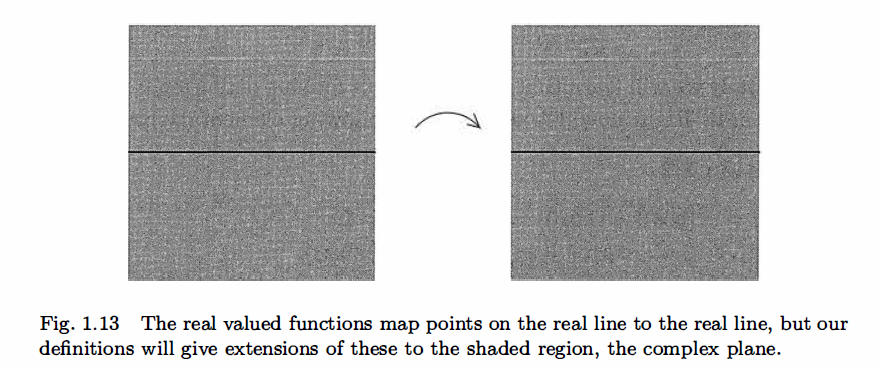
\includegraphics[width=0.7\textwidth]{./SaltChapter/fig-1-13}
\end{center}
\caption{실함수는 실수축 위의 점을 실수축 위로 대응시키는 반면
우리의 정의는 이를 그림자 영역인 복소평면으로 확장한 것이다.}
\label{fig-1-13}
\end{figure}

이러한 확장은  
이는 실수에 한정했을 때 가질 수 없었던 
새롭고 흥미로운 특성을 복소평면에서 보여준다는 것을 앞으로 살펴볼 것이다.
또한 이 함수들은 복소미분 가능함수의 중요한 예로서의 역할도 한다.
지수함수와 삼각함수는 복소평면 위의 모든 점에서 복소미분 가능하며
로그함수는 연속인 점에서 복소미분 가능하다.

우선  지수함수부터 살펴보자.

\subsection{지수함수 $\exp z$} \label{sec-1-4-1}

\begin{saltdefinition}[복소 지수함수] {}{} \label{def-1-2}
$z=x+iy\in \mathbb C$($x,y\in\mathbb R$)에 대하여
복소 지수함수 $\exp z$를 다음과 같이 정의한다.
$$
\exp z = e^x(\cos y +i\sin y).
$$
\end{saltdefinition}

우선 $y=0$일 때, 우변은 $e^x$와 같다. 따라서 이 정의는
일반적인 지수함수 $(\mathbb R \ni) x \mapsto e^x (\in \mathbb R)$의 확장이다.
하지만, 정의는 자연스럽게 보이지 않는다. 
$z\mapsto e^{\Re(z)}$로 정의해도 실수 지수함수의 확장을 얻을 수 있기 때문이다.
이렇게 간단히 정의하면 되는 것을 왜 사용하지 않을까?
우리가 정의한 방식을 쓰는 이유는
실수 지수함수를 복소평면 전체에서 복소미분 가능한 성질을 가지도록
확장하는 유일한 방법이기 때문이다. 
이와 관련하여 
128페이지 %[salt]===> 페이지 번호
예제 4.8 %[salt]===> \ref{example-4-8}
를 참고하라.
실제로 실수 지수함수의 미분공식
$$
\dfrac{d}{dx}e^x  = e^x \quad x\in\mathbb R
$$
과 유사하게 다음이 성립함을 보일 예정이다.
$$
\dfrac{d}{dz} \exp z  = \exp z \quad z\in\mathbb C.
$$
결론적으로 우리는 이상하게 보이는 정의가 실제로 자연스럽다는 것을 공부하게 될 것이다.
지금은 다음과 같은 기본적인 성질부터 확인해보자.

\begin{saltprop} [] {prop-1-2} {}{} %\label{prop-1-2}
\begin{itemize}
\item[(1)] $\exp 0 = e^0(\cos 0 + i\sin 0) = 1\cdot(1+i0) = 1$.
\item[(2)] $z_1, z_2\in \mathbb C$에 대하여, $\exp(z_1+z_2) = (\exp z_1)(\exp z_2)$.
\item[(3)] $z \in \mathbb C$에 대하여, $\exp z \ne 0$ 이고 $(\exp z)^{-1} = \exp (-z)$.
\item[(4)] $z \in \mathbb C$에 대하여, $\exp(z+2\pi i) = \exp z$.
\item[(5)] $z \in \mathbb C$에 대하여, $|\exp z| = e^{\Re(z)}$.
\end{itemize}
\end{saltprop}

{\bf 증명}

\noindent
(2)  $z_1 = x_1 + iy_1$과 $z_2 = x_2 + iy_2$이면,
\begin{align*}
\exp(z_1+z_2)
&= e^{(x_1+x_2) + i(y_1+y_2)} = e^{x_1+x_2}
\left( \cos(y_1+y_2) + i\sin(y_1+y_2) \right) \\
&= e^{x_1}e^{x_2} \left( \cos y_1 \cos y_2 - \sin y_1\sin y_2
+ i(\sin y_1\cos y_2 + \cos y_1\sin y_2) \right) \\
&= e^{x_1} (\cos y_1 + i\sin y_1)  e^{x_2} (\cos y_2 + i\sin y_2)  
= (\exp z_1)(\exp z_2).
\end{align*}
(3) 앞의 식을 쓰면,
$$
1  = \exp 0 = \exp (z-z) = (\exp z)(\exp (-z))
$$
에서 $\exp z \ne 0$이고 $(\exp z)^{-1} = \exp(-z)$을 얻는다.
따라서 $\exp$ 함수는 $\mathbb C$의 원소를 
``뚫린(punctured)'' 평면 $\mathbb C\setminus \{0\}$으로 보낸다.

\noindent
(4) 다음 식으로부터
\begin{align*}
\exp(z+2\pi i)
&= (\exp z)(\exp (2\pi i)) = (\exp z)\cdot e^0(\cos(2\pi) + i\sin(2\pi)) \\
&= (\exp z)\cdot 1\cdot(1+i\cdot 0) = \exp z
\end{align*}
$\exp$ 함수는 ``$y$축 방향으로 주기성''이 있으며, 주기는 $2\pi$임을 알 수 있다.
그림 \ref{fig-1-14}를 보자.

\begin{figure}[!h]
\begin{center}
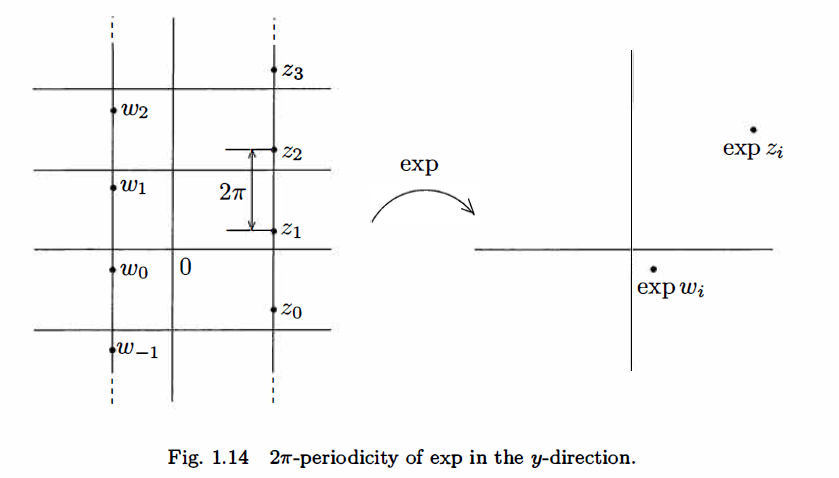
\includegraphics[width=0.6\textwidth]{./SaltChapter/fig-1-14}
\end{center}
\caption{$y$축 방향으로 $2\pi$ 주기를 갖는 복소 지수함수 $\exp$}
\label{fig-1-14}
\end{figure}

이러한 현상은 실수의 성질 갖는 $x$축 방향으로는 나타나지 않는다.
함수 $x\mapsto \exp(x+iy_0)$ ($y_0\in \mathbb R$은 고정하자)는 일대일 함수이다.
그림 \ref{fig-1-15}를 보라.

\begin{figure}[!h]
\begin{center}
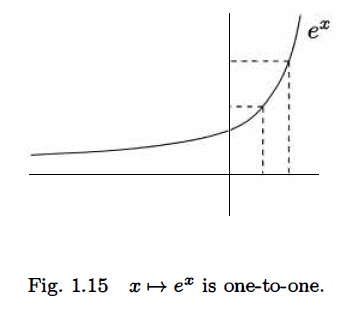
\includegraphics[width=0.3\textwidth]{./SaltChapter/fig-1-15}
\end{center}
\caption{$x\mapsto e^x$는 일대일이다}
\label{fig-1-15}
\end{figure}

\noindent
(5) $x,y \in \mathbb R$에 대하여
$|e^x \cos y + ie^x\sin y| = \sqrt{e^{2x}((\cos y)^2 + (\sin y)^2)} = e^x$.
따라서 $|\exp(x+iy)| = e^x$.
이로부터 $\exp$ 함수는 복소평면의 수직선(실수부가 같은 점들)을
원(절대값이 같은 점, 즉, 원점에서의 거리가 일정한 점)으로 보낸다.
\hfill $\square$

명제 \ref{prop-1-2} (3)은 $\exp$ 함수가 일대일이 아니며
$2\pi i$의 주기를 가짐을 보여준다.
그림 \ref{fig-1-16}은 함수 $z\mapsto \exp z$가
수평선(허수부 $y$가 고정된)과 수직선(실수부 $x$가 고정된)에 작용한 결과를 보여준다.
이는 그림 \ref{fig-1-17}에 표현된 특징을 종합하여 얻을 것이다.

\begin{figure}[!h]
\begin{center}
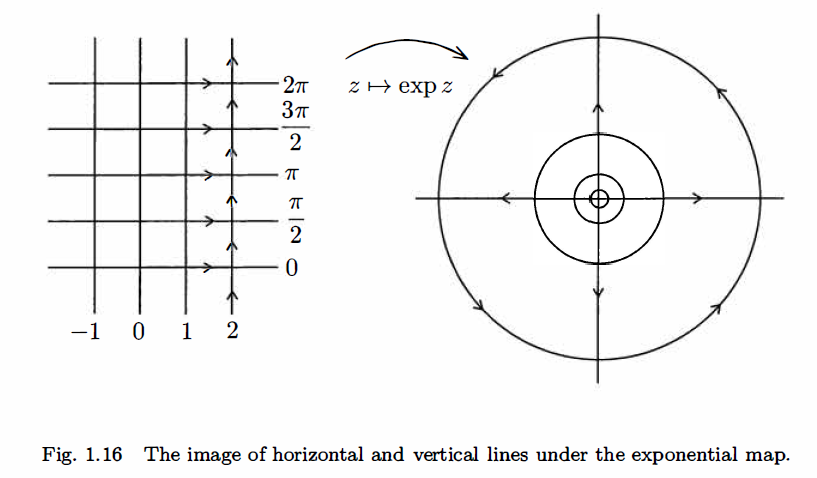
\includegraphics[width=0.6\textwidth]{./SaltChapter/fig-1-16}
\end{center}
\caption{복소 지수함수에 의한 수직선과 수평선의 상(image)}
\label{fig-1-16}
\end{figure}

\begin{figure}[!h]
\begin{center}
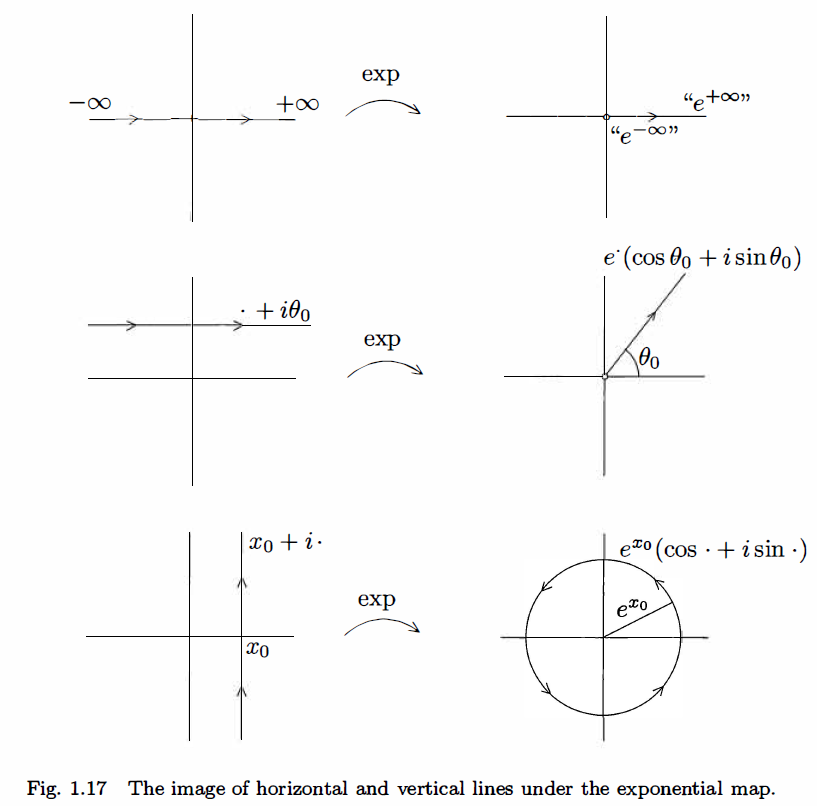
\includegraphics[width=0.6\textwidth]{./SaltChapter/fig-1-17}
\end{center}
\caption{복소 지수함수에 의한 수직선과 수평선의 상(image)}
\label{fig-1-17}
\end{figure}

그림 \ref{fig-1-16}을 보면
$\exp$ 함수는 영역 내 곡선이 이루는 각을 보존함을 알 수 있다.
다시 말하면, 서로 수직인 수평선과 수직선은 서로 수직인 원과 방사형 반직선으로 매핑된다.
뒤에서 우리는 이것은 우연한 것이 아니며, ``등각 특성(conformality)'', 즉, 
두 곡선이 이루는 각도와 함께 ``방향(orientation)''까지 보존하는 것은
영역에 정의된 모든 복소미분 가능함수가 갖는 성질임을 보일 것이다.

{\bf 오일러 공식: }
$z=iy$ ($y\in \mathbb R$)에 대하여
$$
\exp(iy) = \cos y + i \sin y
$$
를 오일러 공식이라 부른다.
따라서 복소수의 극형식은 $z=r(\cos\theta + i\sin\theta) = r\exp(i\theta)$로
다시 쓸 수 있다.

\begin{salt_exercise} \label{ex-1-31}
$z: i\dfrac{9\pi}2, 3+\pi i$에 대하여
$\exp z$를 계산하라.
\end{salt_exercise}

\begin{salt_exercise} \label{ex-1-32}
$\exp z = \pi i$를 만족하는 모든 $z\in\mathbb C$를 찾아라.
\end{salt_exercise}

\begin{salt_exercise} \label{ex-1-33}
곡선 $t\mapsto \exp(it):[0,2\pi] \to \mathbb C$를 그려라.
\end{salt_exercise}

\begin{salt_exercise} \label{ex-1-34}
지수함수 $z=x+iy \mapsto \exp z$가 직선 $y=x$를 어떤 도형으로 보내는지 설명하라.
다음 단계로 진행하면 된다:
우선 매개변수를 $x=t$, $y=t$라 놓고
보낸 이미지의 매개변수방정식을 구하라.
이 곡선을 그리고 $t$가 증가함에 따라, $t\to\pm\infty$에 따라 어떻게 되는지 설명하라.
\end{salt_exercise}

\begin{salt_exercise} \label{ex-1-35}
$z=x+iy$의 실수부와 허수부 $x,y$를 이용하여
$\exp(z^2)$과 $\exp(1/z)$의 절대값, 실수부와 허수부를 구하라.
\end{salt_exercise}


\subsection{삼각함수}\label{sec-1-4-2}

지수함수를 확장한 것과 같이
실수에 정의된 삼각함수를 복소수 삼각함수로 확장해보자.
앞에서 언급한 오일러 공식으로부터 실수 $x$에 대하여 다음 식을 얻는다.
$$
\exp(ix) = \cos x + i \sin x, \quad
\exp(-ix) = \cos x - i \sin x.
$$
이로부터 
$$
\cos x = \dfrac{\exp(ix) + \exp(-ix)}2, \quad
\sin x = \dfrac{\exp(ix) - \exp(-ix)}{2i}
$$
를 얻어 복소수 $z\in\mathbb C$에 까지 확장한 다음 정의를 만들 수 있다.
$$
\cos z = \dfrac{\exp(iz) + \exp(-iz)}2, \quad
\sin z = \dfrac{\exp(iz) - \exp(-iz)}{2i}.
$$
당연히 이 정의는 실수에 정의된 삼각함수의 확장이다.
왜냐 하면, 오일러 공식으로부터 
$z=x$일 때, $\cos z = \cos x$, $\sin z = \sin x$가 됨을 확인할 수 있기 때문이다.

몇가지 삼각함수 공식은 복소수에서도 여전히 유효하다.
예를 들면, $\cos(z_1+z_2) = (\cos z_1)(\cos z_2) - (\sin z_1)(\sin z_2)$는 
다음과 같이 보일 수 있다.
\begin{align*}
(\cos z_1)(\cos z_2) &- (\sin z_1)(\sin z_2)  \\
&= \left( \dfrac{\exp(iz_1)+\exp(-iz_1)}2\right)
\left( \dfrac{\exp(iz_2)+\exp(-iz_2)}2\right) \\
& \quad - \left( \dfrac{\exp(iz_1)-\exp(-iz_1)}{2i}\right)
\left( \dfrac{\exp(iz_2)-\exp(-iz_2)}{2i}\right) \\
&= \dfrac{2\exp(i(z_1+z_2)) + 2\exp(-i(z_1+z_2))}{4} 
= \cos(z_1+z_2).
\end{align*}

\begin{salt_exercise} \label{ex-1-36}
모든 $z_1, z_2 \in \mathbb C$에 대하여
$\sin(z_1+z_2) = (\sin z_1)(\cos z_2) + (\cos z_1)(\sin z_2)$이 성립함을 보여라.
\end{salt_exercise}

$(\sin z)^2 + (\cos z)^2 = 1$도 성립한다.
\begin{align*}
(\sin z)^2 + (\cos z)^2 
&=  \left(\dfrac{\exp(iz)-\exp(-iz)}{2i}\right)^2
+ \left(\dfrac{\exp(iz)+\exp(-iz)}{2}\right)^2 \\
&= \frac{\exp(2iz) - 2 + \exp(-2iz)}{-4}
+ \frac{\exp(2iz) + 2 + \exp(-2iz)}4 \\
&=1.
\end{align*}

하지만, 모든 실수 $x$에 대하여 삼각함수가 
$|\sin x| \le 1$와 $|\cos x|\le 1$를 만족하는 것과 달리
복소수에서 
$z\mapsto \sin z$와 $z\mapsto \cos z$는 유계가 아니다.
$z=iy$($y\in\mathbb R$)에 대하여
$$
\cos (iy) = \frac{\exp(i(iy))+\exp(-i(iy))}2
= \frac{\exp(-y) + \exp(y)}2 = \frac{e^{-y}+e^y}2
$$
이므로
$y\to \pm \infty$일 때, $\cos(iy) \to +\infty$이다.
$$
\sin(iy) = \frac{e^{-y}-e^y}{2i}
$$
이므로 
$y\to \pm \infty$일 때, $|\sin(iy)| \to +\infty$이다.

뒤에서 $z\mapsto \cos z$와 $z\mapsto \sin z$는 
복소평면 위의 모든 점에서 복소미분 가능함을 보일 것이다.


\begin{salt_exercise} \label{ex-1-37}
복소수 $z=x+iy$ ($x,y\in\mathbb R$)에 대하여
$$
\cos z = (\cos x)(\cosh y) - i(\sin x)(\sinh y), \quad
|\cos z|^2 = (\cosh y)^2 - (\sin x)^2
$$
을 증명하라. 단, $\cosh y := \dfrac{e^y+e^{-y}}2$, 
$\sinh y := \dfrac{e^y-e^{-y}}2$이다.
\end{salt_exercise}

\begin{salt_exercise} \label{ex-1-38}
방정식 $\cos x = 3$은 실근 $x$를 갖지 않음은 잘 알려져 있다.
하지만, $\cos z=3$을 만족하는 복소수 $z$는 존재함을 보이고
해를 모두 찾아라.
\end{salt_exercise}

\subsection{로그함수}

실수의 경우,
양수 $y$에 대하여 $\log y\in \mathbb R$은
$e^{\log y} = y$를 만족하는 유일한 실수이다.
따라서 $\log : (0,\infty) \to \mathbb R$은 
함수 $x\mapsto e^x: \mathbb R \to (0,\infty)$의 역함수이다.
그림 \ref{fig-1-18}을 보라.

\begin{figure}[!h]
\begin{center}
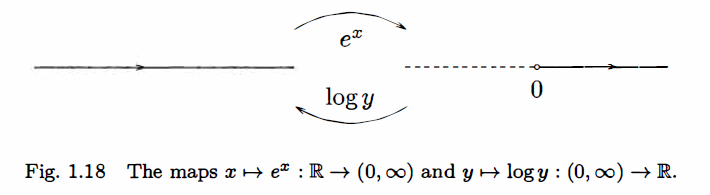
\includegraphics[width=0.8\textwidth]{./SaltChapter/fig-1-18}
\end{center}
\caption{함수 $x\mapsto e^x : \mathbb R \to (0,\infty)$와
$y\mapsto \log y : (0,\infty) \to \mathbb R$}
\label{fig-1-18}
\end{figure}

복소수의 경우,
복소 지수함수는 $\exp: \mathbb C \to \mathbb C\setminus \{0\}$이다.
이제 복소 지수함수의 역함수로서 $\mathbb C\setminus \{0\}$에서 $\mathbb C$로의
``복소 로그함수''가 존재하는지 궁금해진다.
우리는 $z\ne0$에 대하여 $\exp w = z$를 만족하는 복소수 $w$를 찾아
``$z$의 복소 로그값''이라 정의하고자 한다.
그런데  지수함수 $\exp$는 $y$축 방향으로 $2\pi$ 주기임을 알고 있기에
$e^w =z$를 만족하는 하나의 $w$를 찾는다면,
모든 $n\in\mathbb Z$에 대하여 $\exp(w+2\pi i n) = \exp w = z$로부터
무한히 많은 해를 추가로 얻는다.
무한한 값 중에서 어떤 $w$를 $z$의 복소 로그값으로 정해야 할까?
$2\pi$ 폭을 값는 특정 수평띠에 속하는
$w$를 고르는 것으로 비유일성 문제를  해결하고자 한다.
실제로 $0$이 아닌 모든 복소수는 
가능한 수평띠 중 어떤 것을 고르더라도 
수평띠에 속하는 점을 함수 $\exp$로 보낸 값으로 얻을 수 있다.
복소 로그함수를 정의하기 위하여
우리는 (다분히 임의로) 수평띠 $\mathbb S := \{ z\in\mathbb C\,:\, -\pi < Im(z) \le \pi\}$를
선택한다. 그림  \ref{fig-1-19}를 보라.

\begin{figure}[!h]
\begin{center}
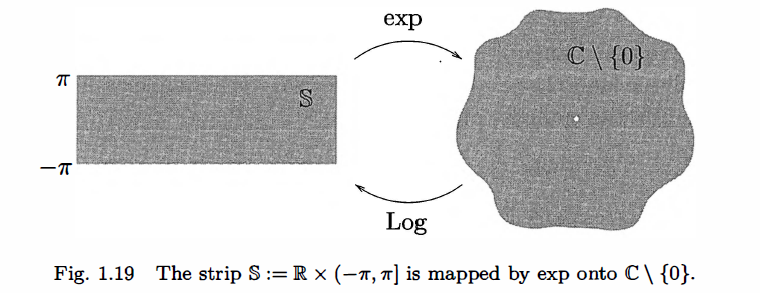
\includegraphics[width=0.8\textwidth]{./SaltChapter/fig-1-19}
\end{center}
\caption{수평띠 $\mathbb S := \mathbb R \times (-\pi, \pi]$에서
$\mathbb C\setminus \{0\}$ 위로의 함수 $\exp$}
\label{fig-1-19}
\end{figure}

이 수평띠에 속하는 $w$ 가운데 $\exp w = z$를 만족하는 것은
유일하게 결정됨을 보일 것이다. 
이를 ``$z$의 주 로그값(principal logarithm)''이라 부르고 $\Log z$라 쓴다.
이를 위해 우선 $0$이 아닌 복소수의 주편각(principal argument)이라는 개념부터 도입한다.

{\bf 복소수의 주편각: }
$z\ne0$에 대하여 다음을 만족하는 실수 $\theta$는 $(-\pi, \pi]$의 범위에서 유일하게 결정된다.
$$
z = |z|(\cos \theta + i\sin\theta).
$$
이 때, $\theta$를 $z$의 주편각이라고 하며, $\Arg z$로 표기한다.
몇가지 예를 들면,
$$
\Arg(3) = 0, \quad \Arg(-1)=\pi, \quad
\Arg(i) = \frac\pi2, \quad \Arg(-i) = - \frac\pi2.
$$
실수축에서 양의 방향 위에 있는 한점을 선택하고
반시계방향으로 원을 그리며 움직이면, 실수축의 음의 방향을 지나갈 때
주편각이 갑자기 점프하는 현상을 볼 수 있다.
실수축의 음수에 대한 주편각은 $\pi$인 반면,
바로 아래쪽에서 다가가는 경우 $-\pi$가 된다.

\begin{salt_exercise}\label{ex-1-39}
복소평면에 집합 $\left\{ z \in\mathbb C \,:\, z\ne0, \dfrac\pi4 < |\Arg(z)| < \dfrac\pi3 \right\}$을
표시하라.
\end{salt_exercise}

이제 $0$이 아닌 복소수에 대한 주 로그값을 정의할 준비가 되었다.

\begin{saltdefinition} {}{} \label{def-1-3}
$z\ne0$에 대하여 주 로그값 $\Log z$는 
$\Log z = \log |z| + i\Arg z$로 정의한다.
\end{saltdefinition}

우선 다음 식을 살펴보자.
\begin{align*}
\exp(\Log z) &= e^{\log |z|} \left( \cos(\Arg z) + i \sin(\Arg z) \right) \\
&= |z| \left( \cos(\Arg z) + i \sin(\Arg z) \right) = z.
\end{align*}
이 식은  $\exp: \mathbb S \to \mathbb C \setminus \{0\}$가 전사함수임을 보여준다.
또한, 일대일 함수도 되는데 왜냐 하면, $z_1, z_2 \in \mathbb S$가 $\exp z_1 = \exp z_2$를 만족한다면,
$\exp(z_1 - z_2) = 1$이 되므로, $z_1 - z_2 = 2\pi ni$($n\in\mathbb Z$)이고,
$z_1, z_2 \in \mathbb S$의 허수부 차이는 $2\pi$ 미만이 되어야 하므로, $n=0$ 즉, 
$z_1 = z_2$이다.

따라서, 두 함수 $\exp : \mathbb S \to \mathbb C \setminus \{0\}$와
$\Log : \mathbb C \setminus \{0\} \to \mathbb S$는 서로 역함수 관계이다.

물론 $0$이 아닌 복소수 $z=|z|e^{i\theta}$의 주편각 $\theta$의 범위를 
$(a, 2\pi +a]$ 또는 $[a, 2\pi+a)$가 되도록 다른 $a$를 선택할 수도 있다.
그러면, 잘 정의된 다른 로그함수를 얻는다(마찬가지로 유효하다).
하지만 이 책에서 $z$의 주 로그값이라 함은 항상 주편각 $\Arg z \in (-\pi, \pi]$를 사용하는
$\log |z| = i\Arg z$를 뜻한다.
예를 들면,
$$
\Log (-i) = \log|-i| + i\Arg(-i) = \log 1 - \dfrac\pi2 i = 0 - \dfrac\pi 2 i = -- \dfrac\pi 2 i.
$$

{\bf $\mathbb C \setminus (-\infty, 0]$에서 $\Log$의 연속성: }
$\Arg : \mathbb C \setminus \{0\} \to (-\pi, \pi]$가 실수축의 음수 부분에서
연속성을 갖지 못하기 때문에 $\Log$는 $\mathbb C \setminus \{0\}$에서 연속함수가 될 수 없다.
즉, $(-\infty, 0)$에 속하는 모든 점에서 연속이 되지 못한다.
$-1$에서 $\Log$가 불연속임을 보이기 위해 $-1$로 수렴하는 다음 수열를 생각하자.
$$
\left( \exp \left( i \left( - \pi + \dfrac 1n \right) \right) \right)_{n\in\mathbb N}.
$$
$$
\lim_{n\to\infty} \exp \left( i \left( -\pi + \frac1n\right) \right) 
= \lim_{n\to\infty} (-1) \left(\cos \frac1n + i \sin \frac1n \right) 
= -1 (1+i0) = -1.
$$
한편,
$$
\Log \left( \exp \left( i \left( -\pi + \frac1n\right) \right) \right)
= \log 1 + i \left( - \pi + \dfrac1n \right) = i\left( - \pi + \dfrac1n \right)
$$
이므로, 다음 두 식은 다른 극한을 갖게 되며
\begin{gather*}
\lim_{n\to\infty}  \Log \left( \exp \left( i \left( -\pi + \frac1n\right) \right) \right)
= i(0 -\pi) = -i\pi, \\
\Log \left( \lim_{n\to\infty} \exp \left( i \left( -\pi + \frac1n\right) \right) \right)
= \Log(-1) = i\pi,
\end{gather*}
결론적으로 $\Log$는 $-1\in\mathbb C \setminus \{0\}$에서 불연속이다.

하지만, 조금 더 작은 정의역 $\mathbb C \setminus (-\infty, 0]$에서 
$\Log$는 연속이다.
이는 주편각 $\Arg(z)$가 $\mathbb C \setminus (-\infty, 0]$에서 연속임을 보이면
바로 얻을 수 있는 결론이다.
증명에 필요한 핵심적인 성질은
$(-\infty,0]$에 속하지 않는 임의의 $z_0$에 대하여
$(-\infty,0]$에 닿지 않는 $z_0$의 근방을 만들 수 있는 여지가 있다는 것이다.
즉, 충분히 작은 $r$을 잡아 원판 $D(z_0, r)$가 
$(-\infty,0]$에 닿지 않도록 할 수 있다.
따라서, 주어진 $\epsilon>0$에 대하여
필요하다면 $r$을 더 줄여서
$D(z_0, r)$에 속하는 모든 $z$가 $|\Arg(z) - \Arg(z_0)|<\epsilon$을 만족하게 할 수 있다.
그림 \ref{fig-1-20}\을 참고하라.

\begin{figure}[!h]
\begin{center}
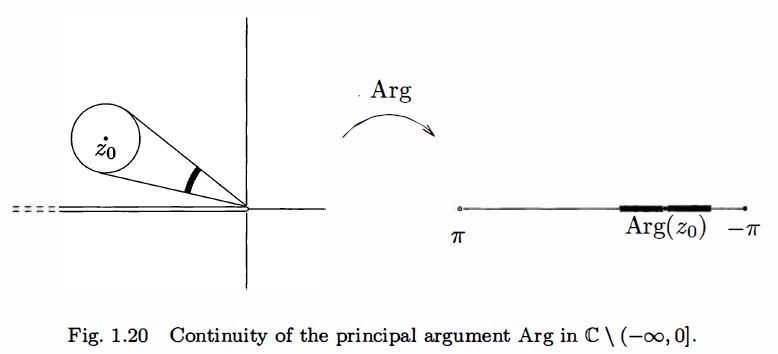
\includegraphics[width=0.8\textwidth]{./SaltChapter/fig-1-20}
\end{center}
\caption{$\mathbb C\setminus (-\infty,0]$에 정의된 주편각 $\Arg$의 연속성}
\label{fig-1-20}
\end{figure}

$\mathbb C \setminus (-\infty,0]$에서 두 함수  $z\mapsto \log |z|$와 $\Arg$가 
연속이므로, $\Log$도 연속이다.

우리는 나중에 $\Log$가 $\mathbb C \setminus (-\infty,0]$에서 연속임을 이용하여
복소미분도 가능함을 보일 것이다.

{\bf $a\in \mathbb C\setminus \{0\}, b\in\mathbb C$에 대하여 $a^b$: }
$a,b$가 복소수이고 $a\ne0$일 때, $a^b$에 대하여 생각해보자.
$a^b$의 주치(principal value)를 다음과 같이 정의한다.
$$
a^b := e^{b\Log(a)}.
$$
예를 들면, $i^i$의 주치는
$$
\exp\left( i\cdot \Log(i) \right)
= \exp \left( i(\log|z| + i\Arg i) \right)
= \exp \left( i \left(0 + i\frac\pi2\right) \right) 
= e^{-\frac\pi2}.
$$

\begin{salt_exercise}\label{ex-1-40}
$\Log (1+i)$를 구하라.
\end{salt_exercise}

\begin{salt_exercise}\label{ex-1-41}
$\Log(-1)$과 $\Log(1)$을 구하라.
$\Log(z^ 2)$은 $2\cdot \Log(z)$와 항상 같지는 않음을 보여라.
\end{salt_exercise}

\begin{salt_exercise}\label{ex-42}
주 로그함수에 의한 원환 $\{ z\,:\, 1 < |z| <e \}$의 상을 구하라.
\end{salt_exercise}

\begin{salt_exercise}\label{ex-43}
$(1+i)^{1-i}$의 주 로그값을 구하라.
\end{salt_exercise}

\section{참고}
복소수의 역사에 대한 설명은 [Needham (1997)]을 인용하였다. %[salt]==> 추후 cite{}로 변경
연습문제 \ref{ex-1-2}\는 [Shastri (2000)]에서, 
연습문제 \ref{ex-1-7},  \ref{ex-1-13}, \ref{ex-1-19}는 [Needham (1997)]에서 가져왔다.
연습문제 \ref{ex-1-23}, 연습문제 \ref{ex-1-34}는 [Beck, Marchesi, Pixton, Sabalka (2008)]을 인용하였다.



